\section{Additional Experiments} \label{apx:exp}
In this section, we describe additional details of the experimental setup; we also
provide and discuss more empirical results, including an empirical analysis of using
a small number of samples to approximate the multilinear extension for the
algorithm of \shortciteS{Ene2020}. 

\subsection{Applications and Datasets}
The cardinality-constrained maximum cut function is defined as follows.
Given graph $G = (V, E)$, and nonnegative edge weight $w_{ij}$ on each edge
$(i,j) \in E$. For $S \subseteq V$, let
$$f(S) = \sum_{i \in V \setminus S} \sum_{j \in S} w_{ij}.$$
In general, this is a non-monotone, submodular function. 

The revenue maximization objective is defined as follows.
Let graph $G = (V, E)$ represent a social network, 
with nonnegative edge weight $w_{ij}$ on each edge
$(i,j) \in E$.
We use the concave graph model introduced by \shortciteS{Hartline2008}.
In this model, each user $i \in V$ is associated with a non-negative,
concave function $f_i: \reals \to \reals$. The value $v_i(S) = f_i( \sum_{j \in S} w_{ij} )$
encodes how likely the user $i$ is to buy a product if the set $S$ has adopted it.
Then the total revenue for seeding a set $S$ is 
$$f(S) = \sum_{i \in V \setminus S} f_i\left( \sum_{j \in S} w_{ij} \right).$$
This is a non-monotone, submodular function. In our implementation,
each edge weight $w_{ij} \in (0,1)$ is chosen uniformly randomly; further,
$f_i( \cdot ) = ( \cdot )^{\alpha_i}$, where $\alpha_i \in (0,1)$ is chosen
uniformly randomly for each user $i \in V$. 

Network topologies from SNAP were used; specifically,
web-Google ($n=875713$, $m = 5105039$), a web graph from
Google, ca-GrQc ($n = 5242, m = 14496$), a collaboration
network from Arxiv General Relativity and Quantum Cosmology,
and ca-Astro ($n = 18772, m = 198110$), a collaboration network
of Arxiv Astro Physics.
In addition, 
a Barabási-Albert random graph was used (BA), with $n = 968$, $m = 5708$.

\subsection{Additional results}
\begin{figure}[ht] \centering
  \subfigure[Objective, BA]{ \label{fig:val-ba}
    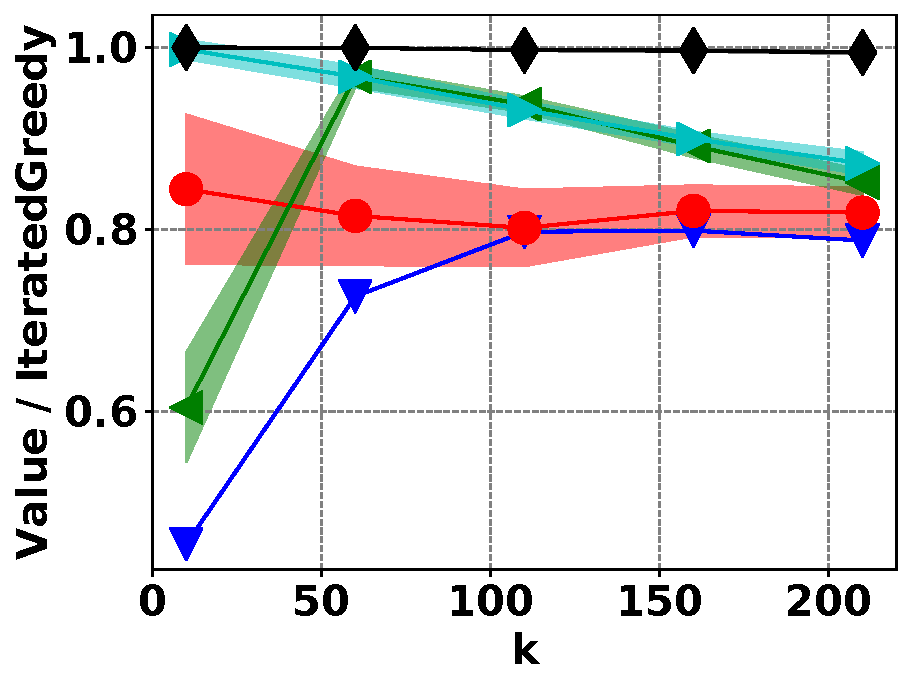
\includegraphics[width=0.28\textwidth,height=0.15\textheight]{plot/BA-val-baseline.pdf}
  }
  \subfigure[Queries, BA]{ \label{fig:query-ba}
    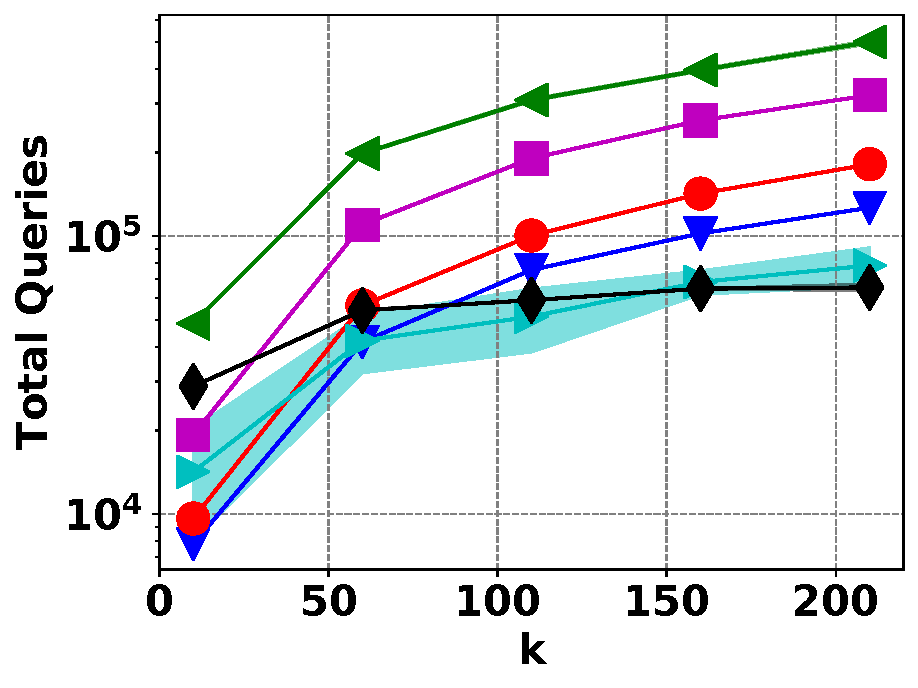
\includegraphics[width=0.28\textwidth,height=0.15\textheight]{plot/BA-query-baseline.pdf}
  }
  \subfigure[Rounds, BA]{ \label{fig:rounds-ba}
    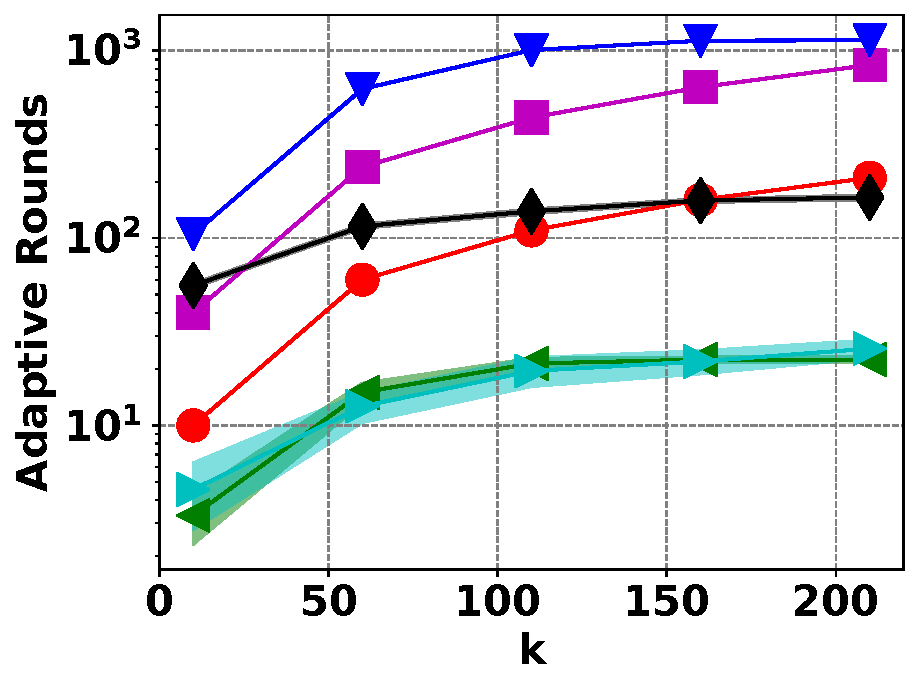
\includegraphics[width=0.28\textwidth,height=0.15\textheight]{plot/BA-round-baseline.pdf}
  }

  \subfigure[Objective, ca-GrQc]{ \label{fig:val-grqc}
    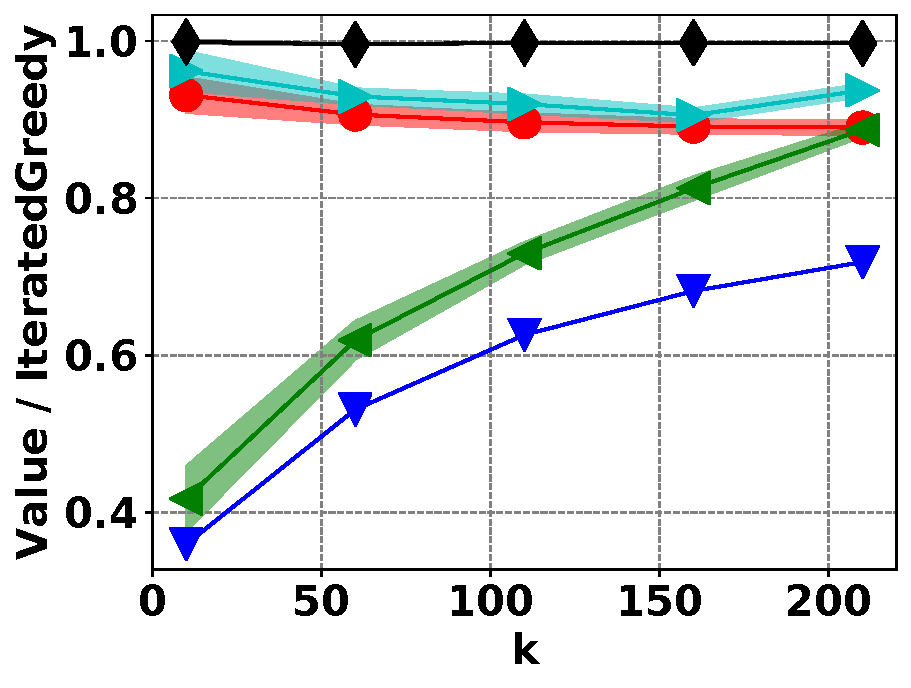
\includegraphics[width=0.28\textwidth,height=0.15\textheight]{plot/grqc-val-smallK-baseline.pdf}
  }
  \subfigure[Queries, ca-GrQc]{ \label{fig:query-grqc}
    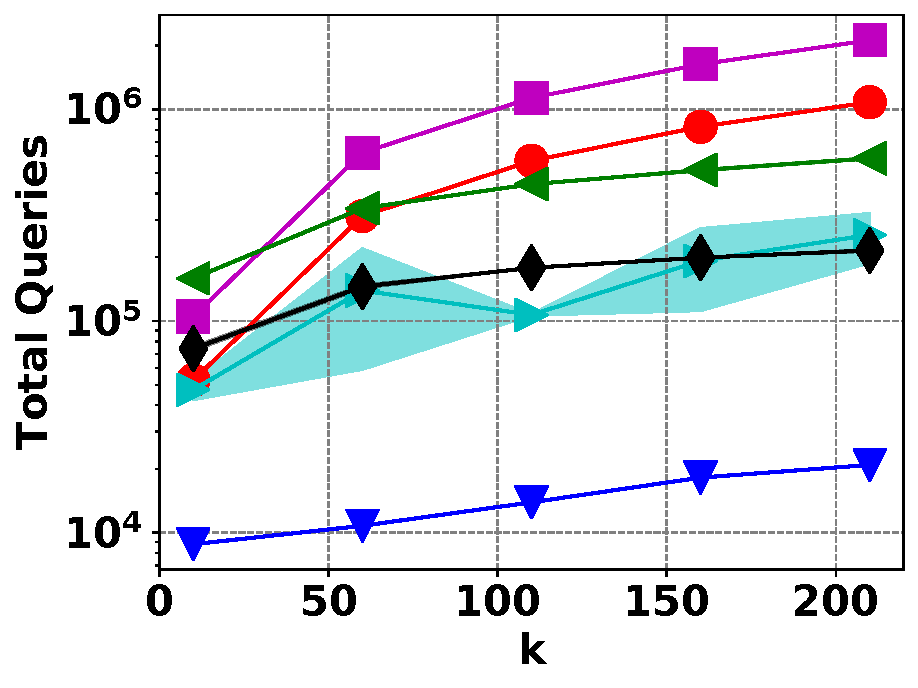
\includegraphics[width=0.32\textwidth,height=0.15\textheight]{plot/grqc-query-smallK-baseline.pdf}
  }
  \subfigure[Rounds, ca-GrQc]{ \label{fig:rounds-grqc}
    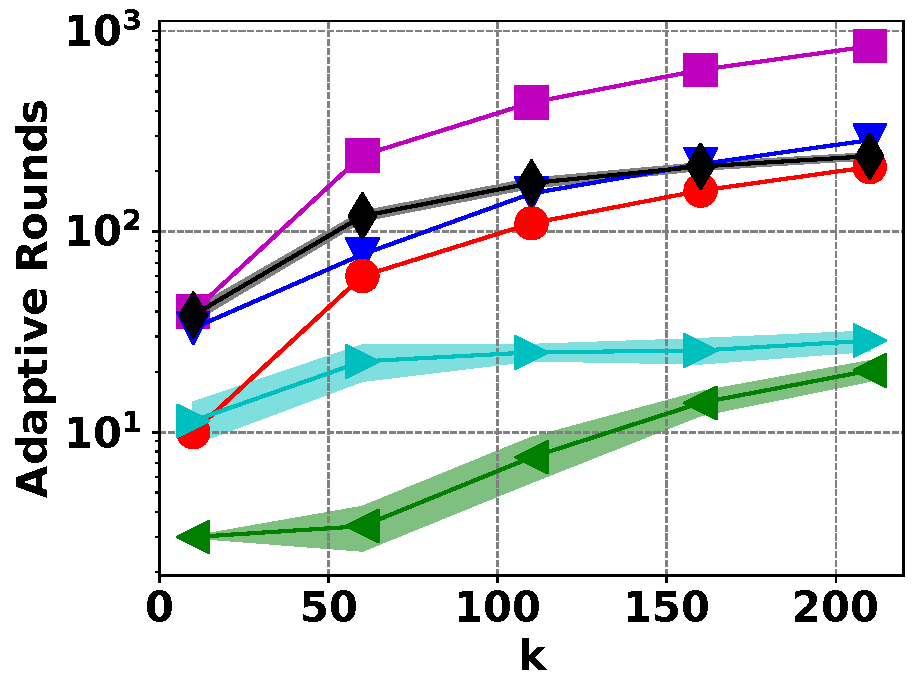
\includegraphics[width=0.32\textwidth,height=0.15\textheight]{plot/grqc-round-smallK-baseline.pdf}
  }
  \caption{Additional results for maximum cut on BA and ca-GrQc. The legend in Fig.~\ref{fig:main} applies.} 
  \label{fig:apx-exp-maxcut}
\end{figure}
\begin{figure}[ht] \centering %%TODO: remove legend from BA plots \centering
  \subfigure[Objective, small $k$]{ \label{fig:val-astro}
    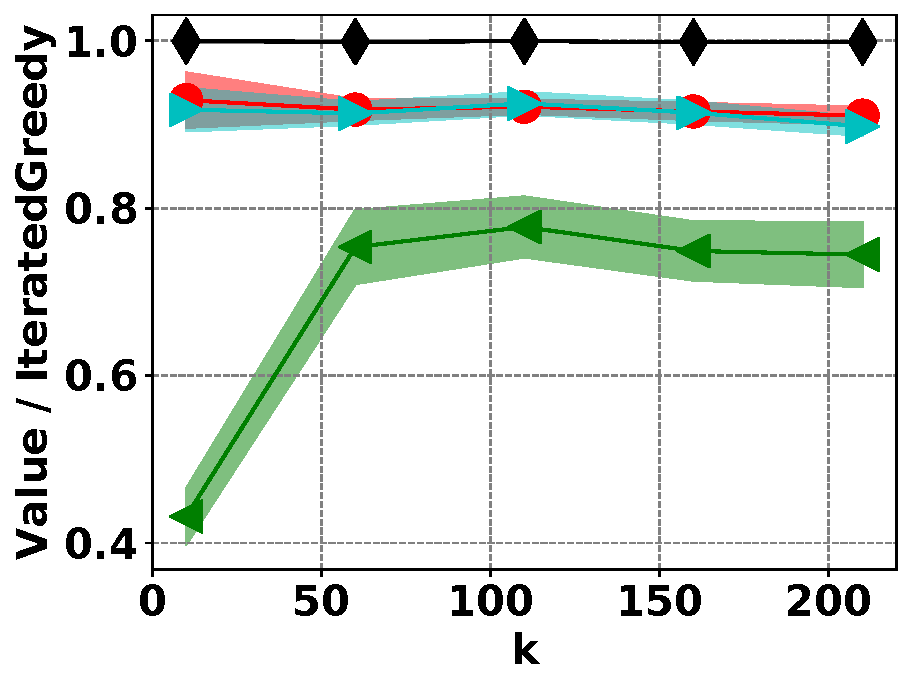
\includegraphics[width=0.28\textwidth,height=0.15\textheight]{plot/astro-val-smallK-baseline.pdf}
  }
  \subfigure[Queries, small $k$]{ \label{fig:query-astro}
    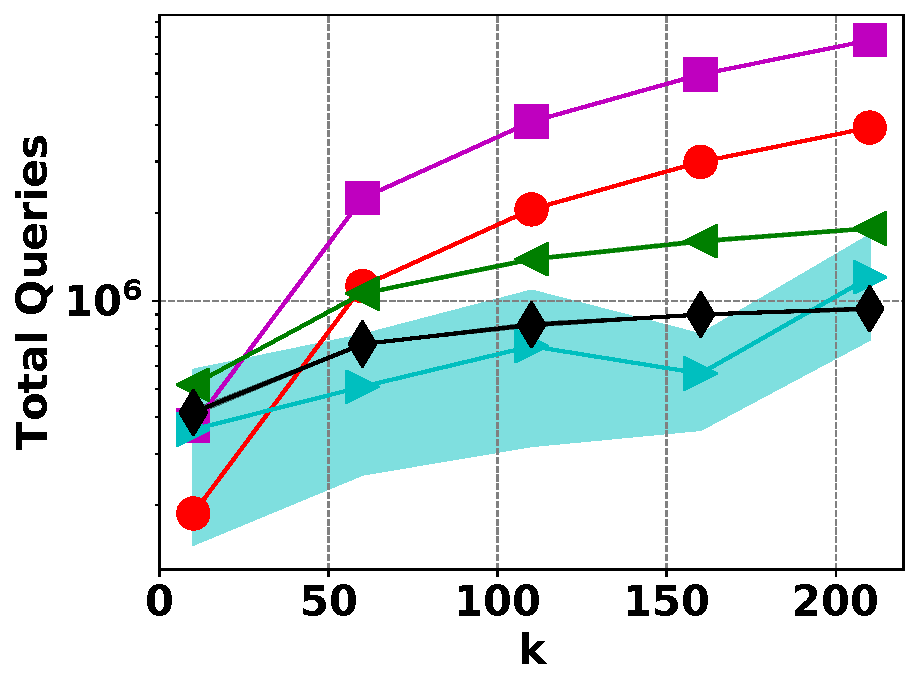
\includegraphics[width=0.28\textwidth,height=0.15\textheight]{plot/astro-query-smallK-baseline.pdf}
  }
  \subfigure[Rounds, small $k$]{ \label{fig:rounds-astro}
    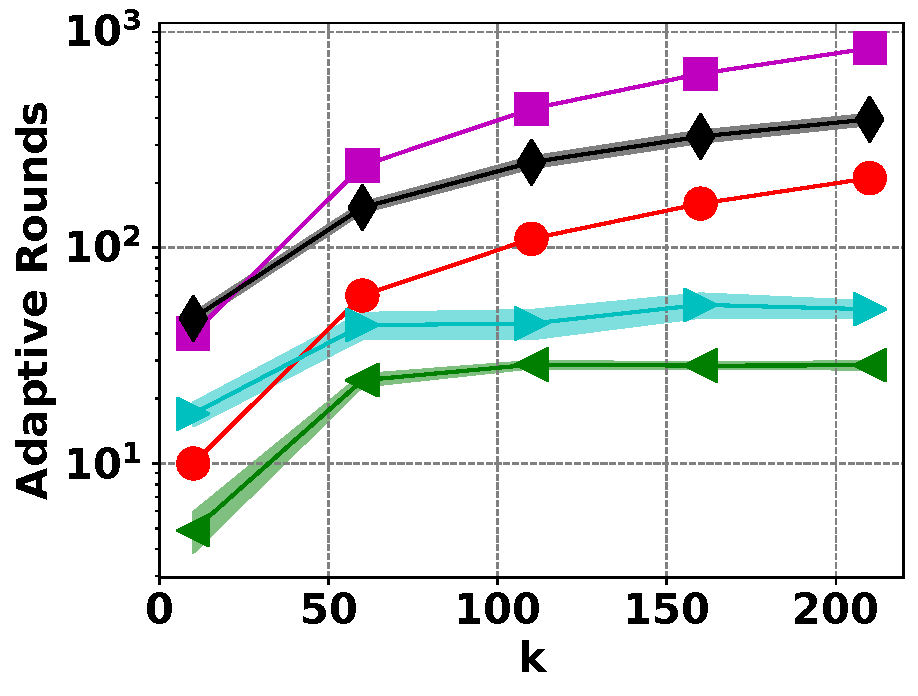
\includegraphics[width=0.28\textwidth,height=0.15\textheight]{plot/astro-round-smallK-baseline.pdf}
  }

  \subfigure[Objective, large $k$]{ \label{fig:val-astro-largek}
    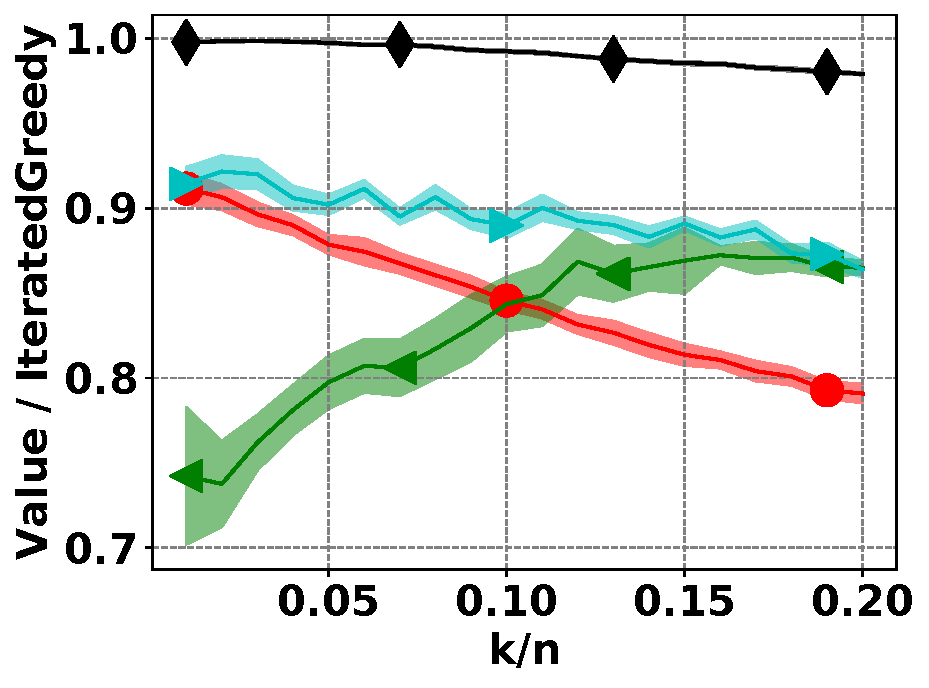
\includegraphics[width=0.28\textwidth,height=0.15\textheight]{plot/astro-val-largeK-baseline.pdf}
  }
  \subfigure[Queries, large $k$]{ \label{fig:query-astro-largek}
    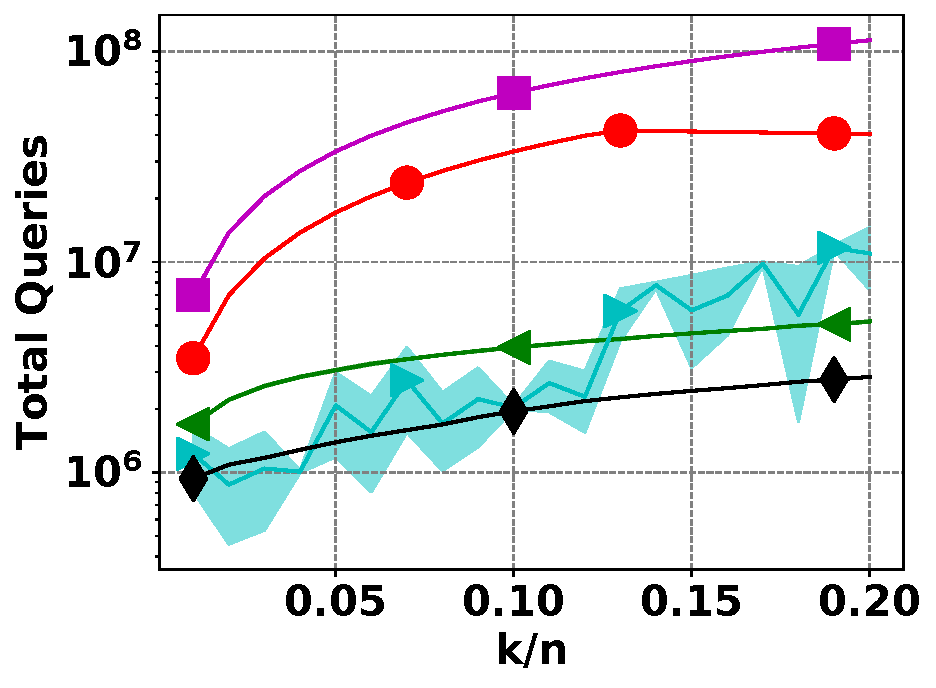
\includegraphics[width=0.28\textwidth,height=0.15\textheight]{plot/astro-query-largeK-baseline.pdf}
  }
  \subfigure[Rounds, large $k$]{ \label{fig:rounds-astro-largek}
    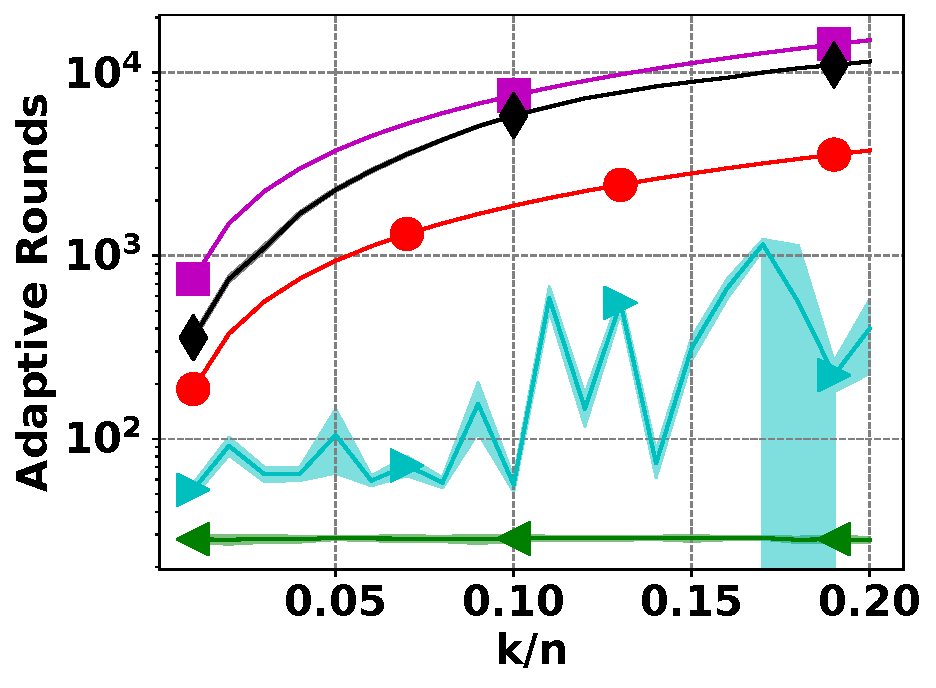
\includegraphics[width=0.28\textwidth,height=0.15\textheight]{plot/astro-round-largeK-baseline.pdf}
  }
  \caption{Results for revenue maximization on ca-Astro, for both small and large $k$ values. Large $k$ values are indicated by a fraction of the total number $n$ of nodes. The legend is the same as in Fig.~\ref{fig:main}.} 
  \label{fig:apx-exp-revmax}
\end{figure}
Results on additional datasets for the maximum cut application are
shown in Figs.~\ref{fig:apx-exp-maxcut}. 
These results are qualitatively
similar to the ones discussed in Section~\ref{sec:exp}. 
For the revenue maximization application, results on ca-Astro are shown
in Figs.~\ref{fig:apx-exp-revmax}, 
for both small and large $k$ values. These results
are qualitatively similar to the results for the maximum cut application. 
%, although
%it should be noted that the low objective value for \anm observed on small $k$ values
%in the maximum cut application extends to larger $k$ values (see Fig.~\ref{fig:val-astro-largek})
%on the revenue maximization application. 

\begin{figure*}[t] \centering
  \subfigure[Objective, BA]{ \label{fig:val-BA-2-atg}
    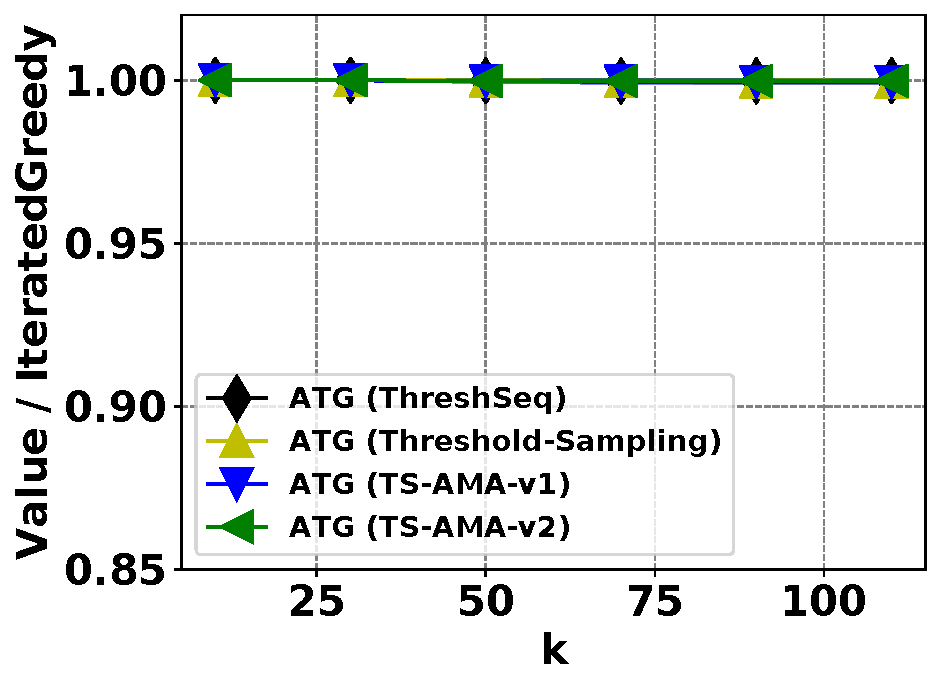
\includegraphics[width=0.3\textwidth,height=0.16\textheight]{plot/BA-val-sample-atg}
  }
  \subfigure[Rounds, BA]{ \label{fig:rounds-BA-2-atg}
    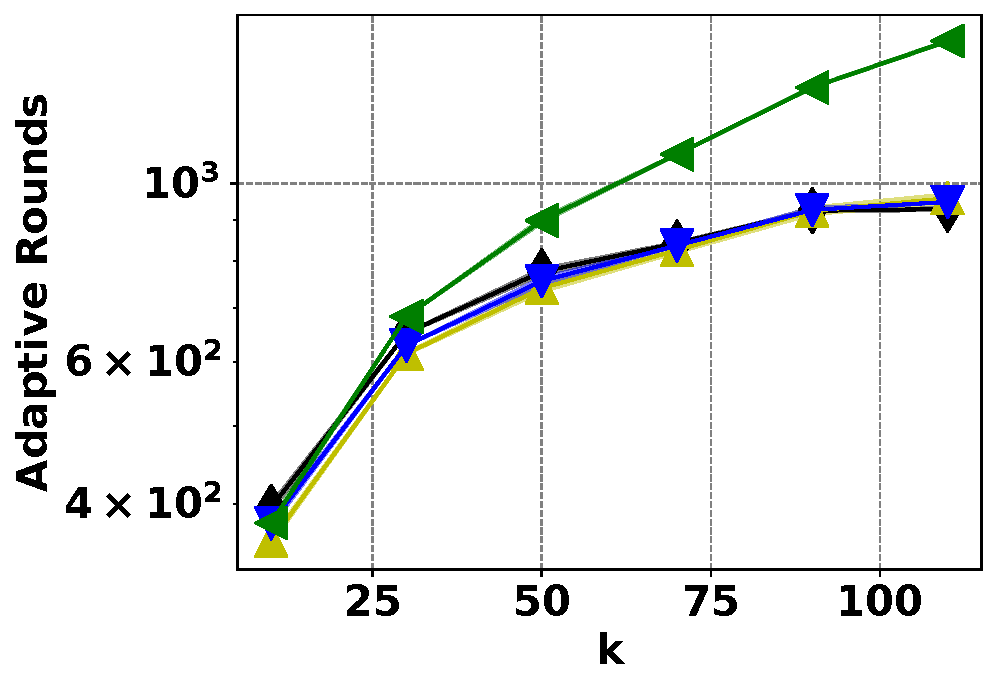
\includegraphics[width=0.3\textwidth,height=0.16\textheight]{plot/BA-round-sample-atg}
  }
  \subfigure[Queries, ca-GrQc]{ \label{fig:query-BA-2-atg}
    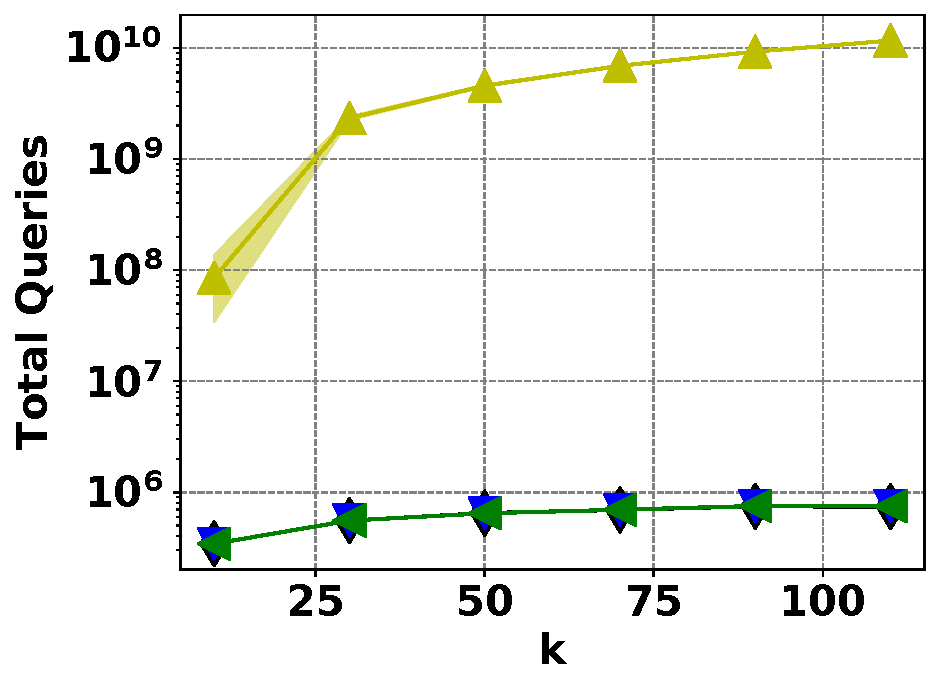
\includegraphics[width=0.3\textwidth,height=0.16\textheight]{plot/BA-query-sample-atg}
  }
  \subfigure[Objective, ca-GrQc]{ \label{fig:val-grqc-2-atg}
    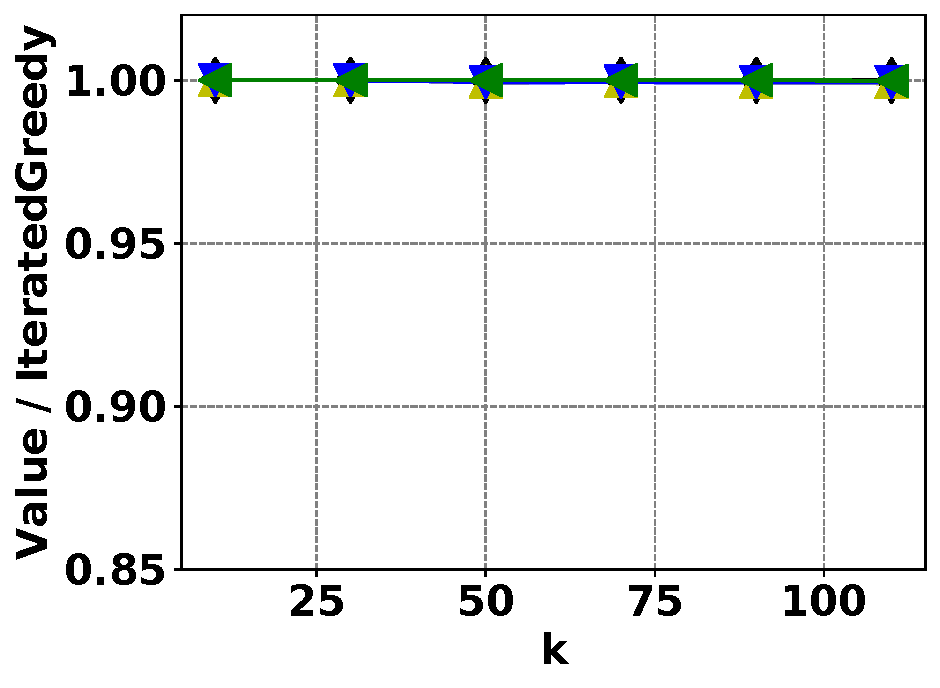
\includegraphics[width=0.3\textwidth,height=0.16\textheight]{plot/grqc-val-sample-atg}
  }
  \subfigure[Rounds, ca-GrQc]{ \label{fig:rounds-grqc-2-atg}
    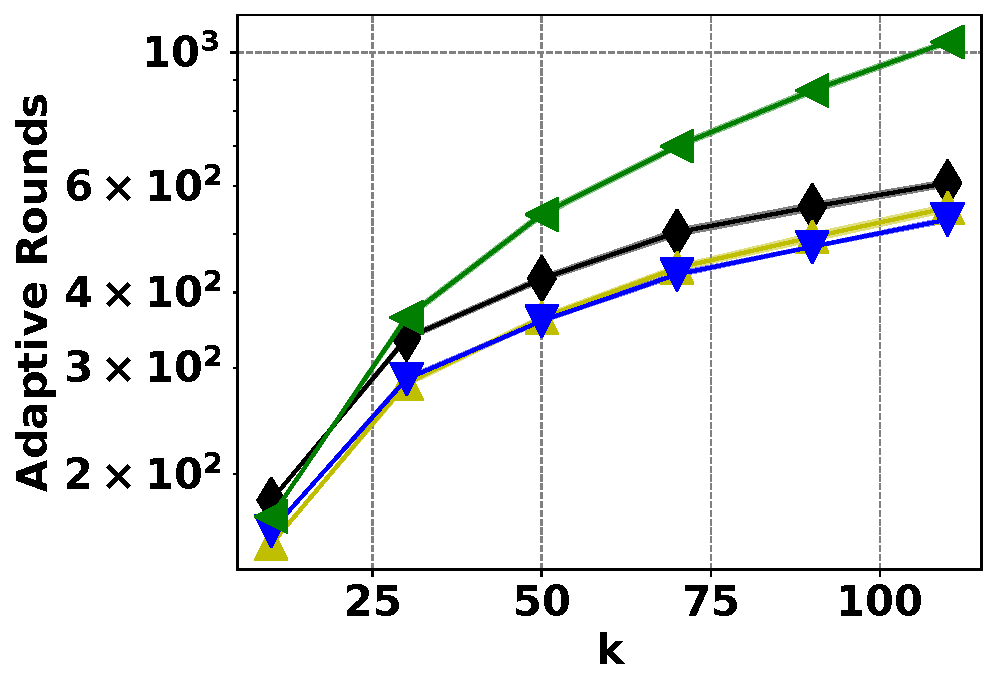
\includegraphics[width=0.3\textwidth,height=0.16\textheight]{plot/grqc-round-sample-atg}
  }
  \subfigure[Queries, ca-GrQc]{ \label{fig:query-grqc-2-atg}
    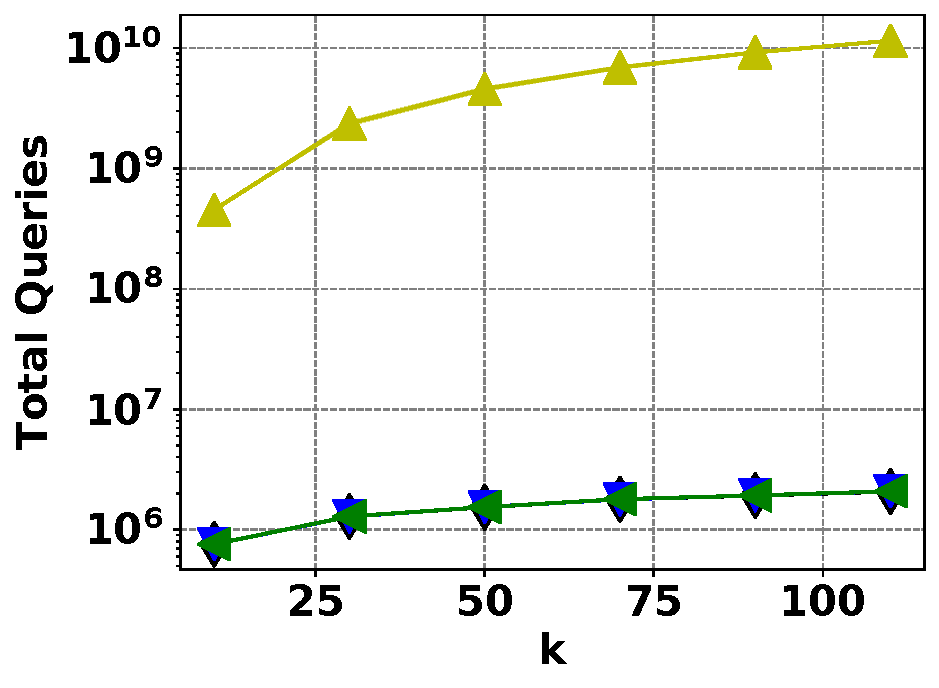
\includegraphics[width=0.3\textwidth,height=0.16\textheight]{plot/grqc-query-sample-atg}
  }
  \caption{Results of \atg and \latg with four threshold procedures on two datasets. 
  The algorithms are run strictly following pseudocode.
   } \label{fig:main3}
\end{figure*}
\textbf{Comparison of \latg with different threshold sampling procedures.}
All \latg algorithms return the competitive solutions compared with \iter;
see Figs.~\ref{fig:val-BA-2-atg} and~\ref{fig:val-grqc-2-atg}.
Since each iteration of \latg calls a threshold sampling subroutine
which is based on the solution of previous iterations and 
a slowly decreasing threshold $\tau$,
after the first filtration of the subroutine, the size of the candidate set is limited.
Thus, there is no significant difference between different {\latg}s
concerning rounds and queries.
However, there are two exceptions.
First, since \tsbin is the only one who has $\oh{\log^2(n)}$ adaptive rounds,
it still runs with more rounds; see Figs.~\ref{fig:rounds-BA-2-atg} and~\ref{fig:rounds-grqc-2-atg}.
Also, the number of queries of \latg with \thresam is significantly large
with the same reason discussed in Section~\ref{sec:exp}.

\begin{figure*}[t] \centering
  \subfigure[Objective value]{ \label{fig:val-Ene}
    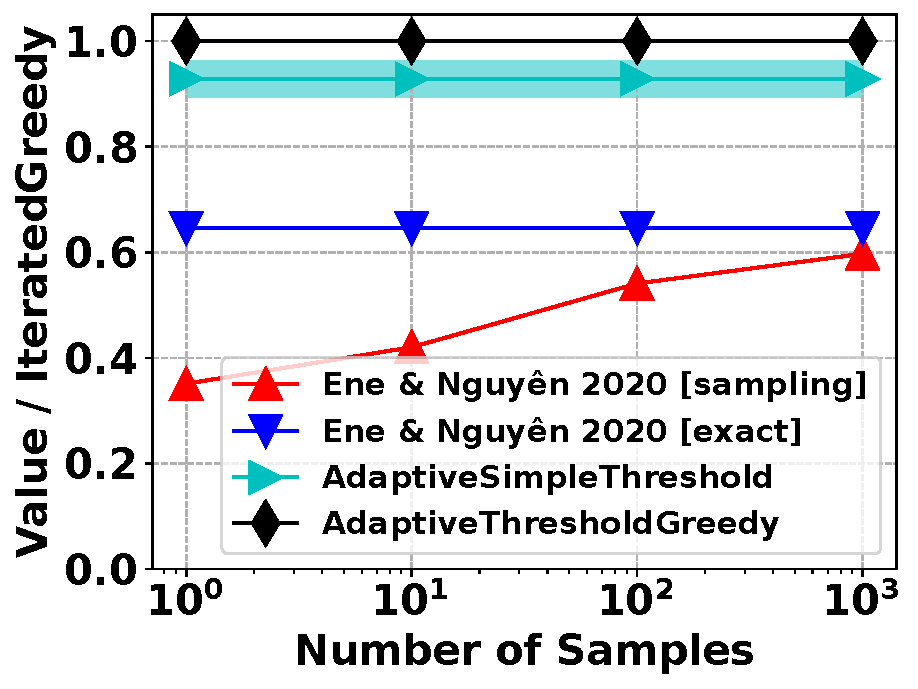
\includegraphics[width=0.28\textwidth,height=0.15\textheight]{plot/ene-val-ba.pdf}
  }
  \subfigure[Queries to set function]{ \label{fig:queryEne}
    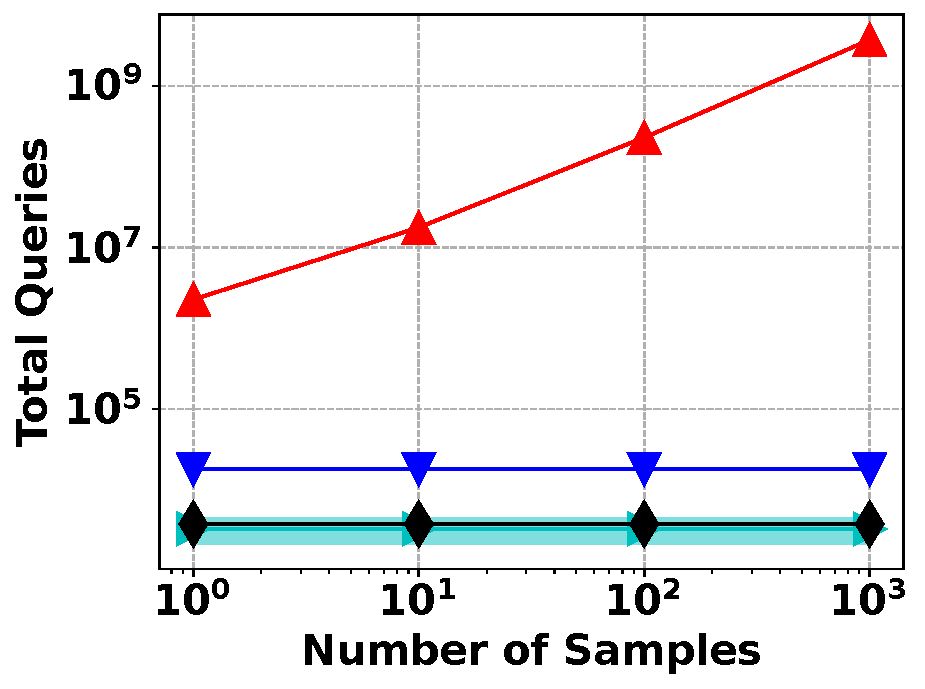
\includegraphics[width=0.28\textwidth,height=0.15\textheight]{plot/ene-query-ba.pdf}
  }
  \subfigure[Adaptive Rounds]{ \label{fig:roundsEne}
    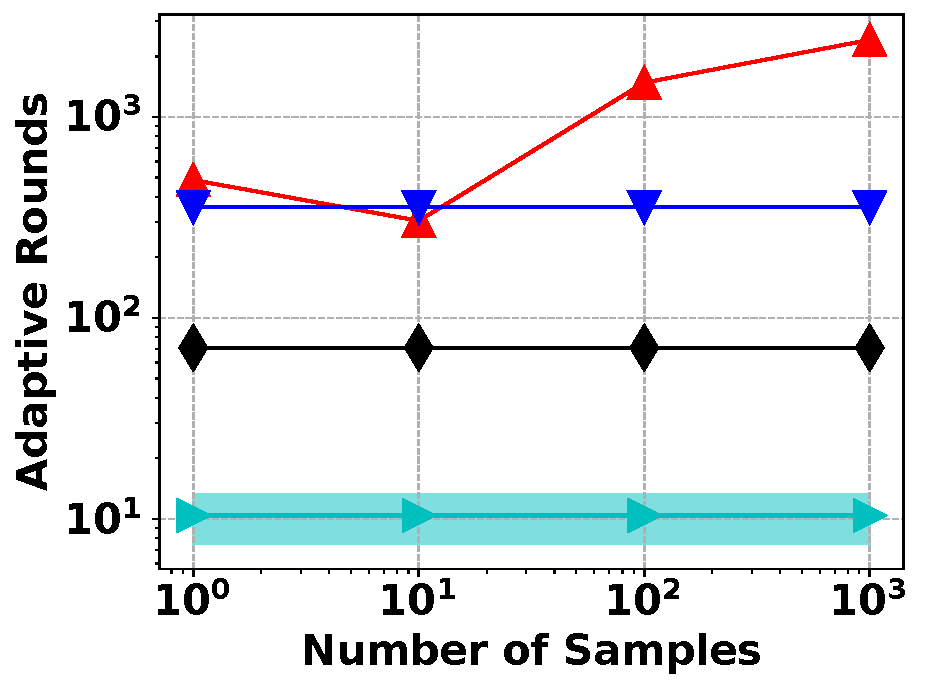
\includegraphics[width=0.28\textwidth,height=0.15\textheight]{plot/ene-rounds-ba.pdf}
  }
  \caption{Comparison of our algorithms with \shortciteS{Ene2020} on a very small random graph ($n = 87$, $k = 10$). In all plots, the $x$-axis shows the number of samples used to approximate the multilinear extension. } \label{fig:multilinear}
\end{figure*} 
\textbf{Approximation of the Multilinear Extension.}
In this section, we further investigate the performance of
\shortciteS{Ene2020} when closed-form evaluation of the multilinear
extension and its gradient are impossible. We find
that sampling to approximate the multilinear extension
and its gradient is extremely inefficient or yields poor solution
quality with a small number of samples. For this reason, we exclude
this algorithm from our revenue maximization experiments.
To perform this evaluation, we compared versions of the
algorithm of \shortciteS{Ene2020} that use varying number
of samples to approximate the multilinear extension.

Results are shown in Fig.~\ref{fig:multilinear} 
on a very small random graph with $n=87$ and $k = 10$.
The figure shows the objective value
and total queries to the set function vs. the number of samples
used to approximate the multilinear extension. 
There is a clear
tradeoff between the solution quality and the number of queries
required; at $10^3$ samples per evaluation, the algorithm
matches the objective value of the version with the 
exact oracle;
however, even at roughly $10^{11}$ queries (corresponding
to $10^4$ samples for each evaluation of the multilinear extension),
the algorithm of \shortciteS{Ene2020} is unable to exceed $0.8$ of
the IteratedGreedy value. On the other hand, if $\le 10$ samples are used to
approximate the multilinear extension, the algorithm is unable to exceed
$0.5$ of the IteratedGreedy value and still requires on the order of $10^7$
queries. 

\subsection{Further Details of Algorithm Implementations}
\label{apx:algimpl}
As stated above, we set $\epsi = 0.1$ for all algorithms
and used $100$ samples to evaluate expectations for adaptive algorithms.
Further, in the algorithms \algOnefullname, \algTwofullname, and \anm,
we ignored the smaller values of $\epsi$, $\delta$ passed to \thresam in each algorithm,
and simply used the input values of $\epsi$ and $\delta$.

For \algTwofullname, we used an early termination condition to check if the threshold
value $\tau < \opt (1 - \epsi ) / (ck)$, by using the best solution value found so far
as a lower bound on $\opt$; this early termination condition is responsible for
the high variance in total queries. We also used a sharper upper bound on $\opt / k$ in place
of the maximum singleton: the sum of the top $k$ singleton values divided by $k$. We
attempted to use the same sharper upper bound in \anm, but it resulted in signficantly worse
objective values, so we simply used the maximum singleton as described in \shortciteS{Fahrbach2018a}.

% Further, we remark that algorithms that use queries to the
% marginal gain of a function are much faster on our applications
% than algorithms that use queries of arbitrary sets. All of the algorithms
% we evaluated can be implemented to use queries of the marginal gain, except for 
% \shortciteS{Ene2020}.

\subsection{Multilinear Extension and Implementation of \shortciteS{Ene2020}} \label{apx:ene}
In this section, we describe the multilinear extension and implmentation of 
\shortciteS{Ene2020}. The multilinear extension $F$
of set function $f$ is defined to be, for $x \in [0,1]^n$:
$$ F(x) = \ex{ f(S) } = \sum_{S \subseteq V} f(S) Pr(S), $$
where $$Pr(S) = \prod_{i \in S} x_i \cdot \prod_{i \not \in S} (1 - x_i).$$
The gradient is approximated by using the central difference in each coordinate
$$ \frac{dg}{dx}(x) \approx \frac{g( x + \gamma / 2 ) - g(x - \gamma /2)}{\gamma}, $$
unless using this approximation required evaluations outside the unit cube, in which
case the forward or backward difference approximations were used. 
The parameter $\gamma$ is set to $0.5$.

Finally, for the maximum cut application, closed forms expressions exist for
both the multilinear extension and its gradient. These are:
$$ F(x) = \sum_{(u,v) \in E} x_u \cdot (1 - x_v ) + x_v \cdot (1 - x_u), $$
and
$$(\nabla F)_u  = \sum_{v \in N(u)} (1 - 2x_v). $$

\textbf{Implementation.} The algorithm was implemented as specified in the pseudocode on page
19 of the arXiv version
of \shortciteS{Ene2020}. We followed the same parameter choices as in
\shortciteS{Ene2020}, although we set $\epsi = 0.1$ as setting it to $0.05$
did not improve the objective value significantly but caused a large increase
in runtime and adaptive rounds. The value of $\delta = \epsi^3$ was used
after communications with the authors. 
